\documentclass[12pt]{article}
\usepackage[margin=1in]{geometry}
\usepackage{setspace}
\usepackage{booktabs}
\usepackage{threeparttable}
\usepackage{caption}
\usepackage{amsmath}
\usepackage{pgfplots}
\pgfplotsset{compat=1.17}
\usepackage[hidelinks]{hyperref}
\onehalfspacing

\title{Voice at the Threshold: Works Councils and Layoffs in Velorian Firms\\[1ex]
\large\textbf{SYNTHETIC TEST PAPER, NOT REAL RESEARCH}}
\author{Anna Kerrow and Tomas Delacourt\\ Veloria School of Management}
\date{}

\begin{document}
\maketitle

\begin{abstract}
\noindent Do works councils change how firms adjust employment? We study the Velorian Workplace Participation Act of 2014, which requires every firm with 250 or more employees to elect a works council with consultation rights over dismissals. Firms with fewer than 250 employees are exempt. Using the national business register and a regression discontinuity design around the 250-employee threshold, we find that firms just above the threshold lay off 2.4 percentage points fewer employees over the three years after the Act than firms just below it. The estimate is stable across bandwidths and kernels, and placebo thresholds show no effect. For firms near the 250-employee threshold, mandated employee voice slows workforce reductions.
\end{abstract}

\noindent\textbf{Keywords:} works councils, employee voice, layoffs, regression discontinuity, labor relations

\newpage

\section{Introduction}

Employee voice is one of the oldest topics in the study of organizations. Workers who can raise concerns inside the firm, rather than exit it, change what managers know and what they can do without consultation. Works councils are the most formal version of this voice. They are elected bodies of employees with legal rights to information and consultation, and in many systems a right to delay or contest dismissals. Scholars of labor relations have long argued that councils make layoffs slower and rarer, because managers must justify reductions to a body that represents the people being dismissed. Scholars of strategy have argued the reverse is also possible: councils may speed up restructuring by giving managers a legitimate channel for hard news.

Evidence on the question is difficult to obtain. Firms with works councils differ from firms without them in size, age, industry, ownership, and the attitudes of their managers. A comparison of the two groups confounds the effect of the council with the effect of whatever led the firm to have one. What is needed is variation in councils that is unrelated to the firm's other traits.

We use a size threshold to obtain this variation. In 2014 the Republic of Veloria passed the Workplace Participation Act, which requires every private firm with 250 or more employees to elect a works council. The council must be consulted before any dismissal of more than five employees within a quarter and may delay such dismissals by up to ninety days. Firms with fewer than 250 employees are exempt. Firms just above and just below the threshold are similar in most respects, but only the former must have a council. We compare them with a regression discontinuity (RD) design (Hahn, Todd, and Van der Klaauw 2001; Lee and Lemieux 2010).

Our data come from the Velorian Business Register, which records the headcount of every registered firm each quarter, and from the Register's dismissal notices, which firms must file for every termination. We measure each firm's headcount on the reference date the Act used to determine coverage and follow its dismissals for three years.

We find that the mandate reduces layoffs. Firms just above the threshold dismiss 2.4 percentage points fewer employees over three years than firms just below it, against a baseline of 8.9 percent. The estimate holds across bandwidths, kernels, and polynomial orders, and placebo thresholds at 200 and 300 employees show no effect. The paper contributes to research on employee voice by providing a design-based estimate of the effect of mandated councils on a central employment outcome, and to research on organizational adjustment by showing that formal consultation rights slow the pace at which firms shed labor.

\section{Institutional Setting}

Veloria is a small open economy with a population of about nine million. Before 2014, works councils were voluntary. Surveys by the Velorian Labour Institute found that about a fifth of firms with more than 100 employees had some form of elected employee committee, but few of these committees had legal standing.

The Workplace Participation Act was passed in February 2014 and took effect on 1 January 2015. Coverage is determined by the firm's registered headcount on 31 December 2013, the reference date. The draft law, including the 250-employee threshold and the reference date, was published in June 2013, and firms could revise their registered headcount for the reference date until 31 March 2014. A firm with 250 or more employees on that date must hold a council election by 30 June 2015. A firm with fewer than 250 employees is exempt for the life of the first council term, which runs to the end of 2017, regardless of later growth. The Register records the date of each council election. Every covered firm in our data held an election by the deadline, and no exempt firm elected a council under the Act, so treatment is a deterministic function of the reference-date headcount.

The council's central right is consultation on dismissals. Before dismissing more than five employees in a quarter, a covered firm must inform the council, provide the business case, and consider alternatives the council proposes. The council may delay the dismissals by up to ninety days. It cannot veto them.

\section{Theory and Hypothesis}

Consultation rights raise the cost of dismissal in two ways. The first is direct. Delay is costly when the reason for a reduction is a fall in demand, because the firm pays wages it would otherwise save. The second is informational. A council that sees the business case can propose alternatives, such as reduced hours, internal transfers, or voluntary departures, that the manager may not have considered or may have rejected as too slow. Both mechanisms point toward fewer dismissals.

A countervailing argument holds that councils can legitimize restructuring. A manager who has consulted may find it easier to carry out reductions without conflict, which could raise dismissals in firms that had been delaying needed adjustments. We expect the first set of mechanisms to dominate in the short run, when the council is new and the firm's managers have little experience working with it.

\medskip
\noindent\textbf{Hypothesis 1 (H1).} \emph{The works-council mandate reduces layoffs.}

\section{Data and Research Design}

\subsection{Sample}

The Velorian Business Register lists every firm with at least one employee. We take all private, for-profit firms that had between 50 and 500 employees on the reference date and that filed accounts for 2012 and 2013. This gives 5,200 firms. We drop public-sector bodies and non-profits because the Act treats them under a separate schedule. Table 1 describes the sample.

\begin{table}[htbp]
\centering
\begin{threeparttable}
\caption{Descriptive statistics}
\begin{tabular}{lrrrr}
\toprule
 & Mean & SD & Min & Max \\
\midrule
Employees on reference date & 142.3 & 97.6 & 50 & 500 \\
Layoff rate, 2015 to 2017 (\%) & 10.3 & 7.9 & 0.0 & 58.4 \\
Layoff rate, 2011 to 2013 (\%) & 10.6 & 8.2 & 0.0 & 61.0 \\
Firm age (years) & 21.4 & 14.2 & 1 & 96 \\
Manufacturing (share) & 0.38 & 0.49 & 0 & 1 \\
Exporter (share) & 0.29 & 0.45 & 0 & 1 \\
Union density, 2012 & 0.22 & 0.19 & 0.00 & 0.91 \\
Revenue per worker, 2012 (thousand crowns) & 184.6 & 121.3 & 22.4 & 1,412.0 \\
\bottomrule
\end{tabular}
\begin{tablenotes}\footnotesize
\item \emph{Notes:} 5,200 private firms with 50 to 500 employees on 31 December 2013. Layoff rate is dismissals filed with the Register over the three calendar years divided by headcount on the reference date.
\end{tablenotes}
\end{threeparttable}
\end{table}

\subsection{Outcome}

The outcome is the layoff rate: the number of dismissals the firm filed with the Register from January 2015 through December 2017, divided by its headcount on the reference date, in percent. Dismissals for cause and retirements are recorded separately in the Register and are excluded. This is the only outcome we use to test H1.

\subsection{Estimation}

The running variable is the firm's headcount on the reference date, centered at 250. Treatment is an indicator for a headcount of 250 or more. We estimate
\begin{equation}
y_i = \alpha + \tau D_i + \beta_1 (x_i - 250) + \beta_2 D_i (x_i - 250) + \varepsilon_i,
\end{equation}
where $y_i$ is the layoff rate, $x_i$ is headcount, and $D_i = \mathbf{1}[x_i \geq 250]$. The coefficient $\tau$ is the discontinuity in the layoff rate at the threshold. We estimate the equation by local linear regression with a triangular kernel within a window of 15 employees on either side of the threshold, that is, for firms with 235 to 265 employees. Some specifications add two-digit industry fixed effects and region fixed effects.

Employee counts are integers, so the running variable is discrete. We cluster standard errors at each value of the running variable following Lee and Card (2008), which yields 31 clusters within the main window and accounts for the discreteness of the running variable.

\section{Results}

\subsection{Validity of the design}

The design requires that firms could not precisely sort themselves to one side of the threshold. Firms that wished to avoid the mandate had an incentive to report fewer than 250 employees on the reference date. We test for such sorting by examining the density of the running variable at the threshold using the local polynomial density test of Cattaneo, Jansson, and Ma (2020). The density test (p = 0.03) shows no significant manipulation around the threshold. Appendix Table A1 reports the number of firms at each headcount near the threshold.

The design also requires that firms on either side of the threshold be similar in traits determined before the Act. Table 2 reports discontinuities in six pre-treatment covariates, estimated with the same local linear specification within a window of 40 employees on either side of the threshold. Five of the six covariates show no discontinuity. Firm age differs at the threshold, which we attribute to chance given the number of covariates tested. Taken together, the covariates are balanced at the threshold.

\begin{table}[htbp]
\centering
\begin{threeparttable}
\caption{Covariate balance at the threshold}
\begin{tabular}{lcc}
\toprule
Covariate & Discontinuity & Mean below threshold \\
\midrule
Firm age (years) & 6.1*** & 24.8 \\
 & (1.9) & \\
Manufacturing (share) & 0.03 & 0.41 \\
 & (0.06) & \\
Exporter (share) & 0.02 & 0.33 \\
 & (0.05) & \\
Union density, 2012 & 0.01 & 0.24 \\
 & (0.03) & \\
Revenue per worker, 2012 & 1.8 & 191.2 \\
 & (3.9) & \\
Layoff rate, 2011 to 2013 (\%) & $-$0.3 & 9.2 \\
 & (0.9) & \\
\midrule
Window (employees) & \multicolumn{2}{c}{$\pm$40} \\
Clusters (running-variable values) & \multicolumn{2}{c}{81} \\
\bottomrule
\end{tabular}
\begin{tablenotes}\footnotesize
\item \emph{Notes:} Each row is a separate local linear regression of the covariate on the treatment indicator and the centered running variable, interacted, with a triangular kernel, for firms with 210 to 290 employees. Standard errors clustered by value of the running variable in parentheses. *** $p<0.01$, ** $p<0.05$, * $p<0.10$.
\end{tablenotes}
\end{threeparttable}
\end{table}

\subsection{Main results}

Figure 1 plots the layoff rate against headcount near the threshold. The binned means fall at the threshold, and the local linear fits on each side show a drop of 2.4 percentage points at 250 employees.

\begin{figure}[htbp]
\centering
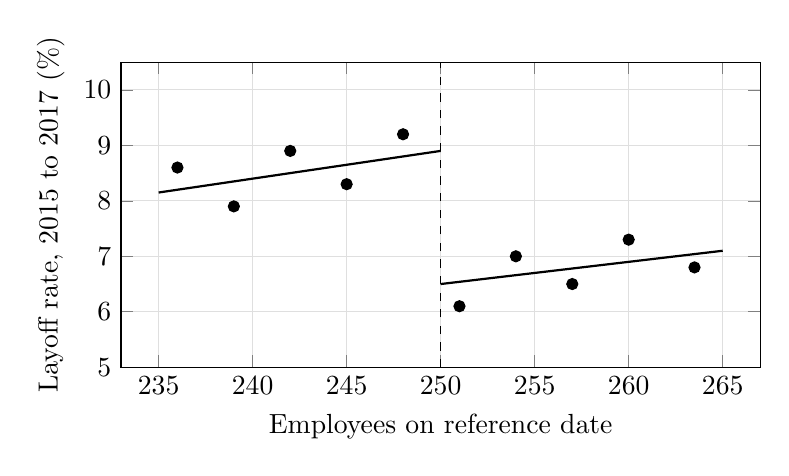
\begin{tikzpicture}
\begin{axis}[
  width=0.8\textwidth, height=0.45\textwidth,
  xlabel={Employees on reference date},
  ylabel={Layoff rate, 2015 to 2017 (\%)},
  xmin=233, xmax=267, ymin=5, ymax=10.5,
  xtick={235,240,245,250,255,260,265},
  ytick={5,6,7,8,9,10},
  grid=major, grid style={gray!25}
]
\addplot[only marks, mark=*, mark size=2pt] coordinates {
  (236,8.6) (239,7.9) (242,8.9) (245,8.3) (248,9.2)
};
\addplot[only marks, mark=*, mark size=2pt] coordinates {
  (251,6.1) (254,7.0) (257,6.5) (260,7.3) (263.5,6.8)
};
\addplot[thick, domain=235:250, samples=2] {8.9 + 0.05*(x-250)};
\addplot[thick, domain=250:265, samples=2] {6.5 + 0.04*(x-250)};
\draw[dashed] (axis cs:250,5) -- (axis cs:250,10.5);
\end{axis}
\end{tikzpicture}
\caption{Layoff rate by headcount near the threshold. Dots are binned means; the number and width of bins (five bins on each side, each three employees wide except the last bin above the threshold, which spans four) are chosen by the mimicking-variance selector of Calonico, Cattaneo, and Titiunik (2015). Lines are local linear fits with a triangular kernel within 15 employees of the threshold. The fitted values at the threshold are 8.9 percent below and 6.5 percent above, a jump of $-$2.4 percentage points, equal to the estimate in Table 3, column 1.}
\end{figure}

Table 3 reports the estimates. In column 1, the layoff rate is 2.4 percentage points lower for firms just above the threshold. Adding industry fixed effects in column 2 and region fixed effects in column 3 changes the estimate little. Relative to the mean of 8.9 percent just below the threshold, the mandate reduces layoffs by about a quarter. The results support H1.

\begin{table}[htbp]
\centering
\begin{threeparttable}
\caption{Effect of the works-council mandate on the layoff rate}
\begin{tabular}{lccc}
\toprule
 & (1) & (2) & (3) \\
\midrule
Above threshold & $-$2.4** & $-$2.3** & $-$2.5** \\
 & (1.1) & (1.0) & (1.0) \\
\midrule
Industry fixed effects & No & Yes & Yes \\
Region fixed effects & No & No & Yes \\
Window (employees) & $\pm$15 & $\pm$15 & $\pm$15 \\
Kernel & Triangular & Triangular & Triangular \\
Polynomial & Linear & Linear & Linear \\
Mean below threshold & 8.9 & 8.9 & 8.9 \\
Clusters & 31 & 31 & 31 \\
Observations & 5,200 & 5,200 & 5,200 \\
\bottomrule
\end{tabular}
\begin{tablenotes}\footnotesize
\item \emph{Notes:} N = 5,200. Dependent variable: layoff rate from 2015 to 2017, in percent. Local linear regression within 15 employees of the 250-employee threshold. Standard errors clustered by value of the running variable in parentheses. *** $p<0.01$, ** $p<0.05$, * $p<0.10$.
\end{tablenotes}
\end{threeparttable}
\end{table}

\subsection{Robustness}

Table 4 examines sensitivity to the bandwidth, the kernel, the polynomial order, and heaping at the threshold. The mean squared error (MSE) optimal bandwidth from the selector of Calonico, Cattaneo, and Titiunik (2014) is 18.4 employees. Columns 1 to 3 use a triangular kernel at this bandwidth, at half of it (9.2), and at double it (36.8). Columns 4 to 6 repeat these with a uniform kernel. Column 7 fits a local quadratic at the MSE-optimal bandwidth. Because 250 is a round number and headcounts may be heaped there, column 8 drops firms with 249 to 251 employees (a donut) and re-estimates at the MSE-optimal bandwidth.

The point estimates range from $-$2.1 to $-$2.9 and are negative in every column. They are more precise at double the bandwidth and less precise at half the bandwidth and with the quadratic. The estimate with a uniform kernel at half the bandwidth (column 5) is not significant at the 10 percent level; the others are significant at the 10 percent level or better. Dropping firms at and next to the threshold leaves the estimate nearly unchanged ($-$2.3 against $-$2.4). The size of the effect does not depend on these choices, though precision does.

\begin{table}[htbp]
\centering
\small
\begin{threeparttable}
\caption{Sensitivity to bandwidth, kernel, polynomial order, and heaping}
\begin{tabular}{lcccccccc}
\toprule
 & (1) & (2) & (3) & (4) & (5) & (6) & (7) & (8) \\
\midrule
Above threshold & $-$2.4** & $-$2.7* & $-$2.2*** & $-$2.5** & $-$2.9 & $-$2.1*** & $-$2.6* & $-$2.3* \\
 & (1.0) & (1.6) & (0.7) & (1.1) & (1.8) & (0.7) & (1.5) & (1.2) \\
\midrule
Bandwidth & 18.4 & 9.2 & 36.8 & 18.4 & 9.2 & 36.8 & 18.4 & 18.4 \\
Kernel & Tri. & Tri. & Tri. & Unif. & Unif. & Unif. & Tri. & Tri. \\
Polynomial & Lin. & Lin. & Lin. & Lin. & Lin. & Lin. & Quad. & Lin. \\
Donut (249 to 251) & No & No & No & No & No & No & No & Yes \\
Clusters & 37 & 19 & 73 & 37 & 19 & 73 & 37 & 34 \\
\bottomrule
\end{tabular}
\begin{tablenotes}\footnotesize
\item \emph{Notes:} Dependent variable: layoff rate from 2015 to 2017, in percent. The bandwidth in column 1 is the MSE-optimal bandwidth for a local linear fit with a triangular kernel; columns 2 and 3 use half and double it. Tri.\ is triangular, Unif.\ is uniform. Standard errors clustered by value of the running variable in parentheses. *** $p<0.01$, ** $p<0.05$, * $p<0.10$.
\end{tablenotes}
\end{threeparttable}
\end{table}

\subsection{Placebo thresholds}

If the estimate reflects the mandate rather than a general pattern in how layoffs vary with firm size, there should be no discontinuity at thresholds where no rule changes. Table 5 applies the main specification (local linear, triangular kernel, a window of 15 employees on each side) at placebo thresholds of 200 and 300 employees. The windows run from 185 to 215 and from 285 to 315, so neither includes firms at the true threshold, and each uses firms from only one side of it. Both estimates are small and far from significant.

\begin{table}[htbp]
\centering
\begin{threeparttable}
\caption{Placebo thresholds}
\begin{tabular}{lcc}
\toprule
 & (1) & (2) \\
 & Threshold 200 & Threshold 300 \\
\midrule
Above placebo threshold & 0.3 & $-$0.4 \\
 & (1.2) & (1.4) \\
\midrule
Window (employees) & 185 to 215 & 285 to 315 \\
Clusters & 31 & 31 \\
\bottomrule
\end{tabular}
\begin{tablenotes}\footnotesize
\item \emph{Notes:} Dependent variable: layoff rate from 2015 to 2017, in percent. Local linear regression with a triangular kernel within 15 employees of each placebo threshold. Standard errors clustered by value of the running variable in parentheses. *** $p<0.01$, ** $p<0.05$, * $p<0.10$.
\end{tablenotes}
\end{threeparttable}
\end{table}

\section{Discussion}

The results show that firms required to elect a works council dismissed fewer employees in the first three years of the council's existence. The effect is about a quarter of the baseline layoff rate. This is large relative to the ninety-day delay the council can impose, which suggests that the informational mechanism matters: councils appear to change which reductions managers pursue, not only when they carry them out.

The findings speak to the debate between labor-relations and strategy accounts of employee voice. The labor-relations view predicts fewer dismissals, and that is what we find. The strategy view, that councils legitimize restructuring, may apply over a longer horizon than we observe. The first council term ends in 2017, and a firm's second council may behave differently once managers and representatives have learned to work together.

Appendix B adds supporting evidence from a different source of variation in employee voice: close shareholder votes on proposals to create a rotating employee seat on the board. Firms where such a proposal narrowly passed also reduced layoffs, which suggests that the effect of voice is not specific to the council form.

The study has limits. We observe dismissals filed with the Register, which excludes departures that firms arrange as voluntary. If councils shift reductions from dismissals to negotiated departures, our estimate overstates the fall in total separations. We also cannot observe the content of council consultations. Future work with meeting records could show which alternatives councils propose and which managers accept.

\section{Conclusion}

Mandated works councils slow the pace at which firms shed labor. Using the 250-employee threshold of the Velorian Workplace Participation Act, we find that firms required to elect a council dismissed 2.4 percentage points fewer employees over three years than firms just exempt from the requirement. The evidence indicates that the mandate reduces layoffs across the economy, and that policy makers weighing participation rules should expect them to dampen employment adjustment in firms of every size.

\section*{References}
\begin{list}{}{\leftmargin=1.5em \itemindent=-1.5em \itemsep=0.3em \parsep=0pt}
\item Calonico, S., Cattaneo, M. D., and Titiunik, R. (2014). Robust nonparametric confidence intervals for regression-discontinuity designs. \emph{Econometrica}, 82(6), 2295--2326.
\item Calonico, S., Cattaneo, M. D., and Titiunik, R. (2015). Optimal data-driven regression discontinuity plots. \emph{Journal of the American Statistical Association}, 110(512), 1753--1769.
\item Cattaneo, M. D., Jansson, M., and Ma, X. (2020). Simple local polynomial density estimators. \emph{Journal of the American Statistical Association}, 115(531), 1449--1455.
\item Cu\~nat, V., Gin\'e, M., and Guadalupe, M. (2012). The vote is cast: The effect of corporate governance on shareholder value. \emph{Journal of Finance}, 67(5), 1943--1977.
\item Hahn, J., Todd, P., and Van der Klaauw, W. (2001). Identification and estimation of treatment effects with a regression-discontinuity design. \emph{Econometrica}, 69(1), 201--209.
\item Lee, D. S., and Card, D. (2008). Regression discontinuity inference with specification error. \emph{Journal of Econometrics}, 142(2), 655--674.
\item Lee, D. S., and Lemieux, T. (2010). Regression discontinuity designs in economics. \emph{Journal of Economic Literature}, 48(2), 281--355.
\end{list}

\clearpage
\appendix
\section*{Appendix A: Distribution of the running variable}

\begin{table}[htbp]
\centering
\begin{threeparttable}
\caption*{Table A1: Number of firms by headcount on the reference date, 235 to 265 employees}
\begin{tabular}{cc@{\hspace{3em}}cc@{\hspace{3em}}cc}
\toprule
Employees & Firms & Employees & Firms & Employees & Firms \\
\midrule
235 & 2 & 246 & 3 & 256 & 1 \\
236 & 2 & 247 & 3 & 257 & 2 \\
237 & 3 & 248 & 4 & 258 & 2 \\
238 & 2 & 249 & 5 & 259 & 1 \\
239 & 2 & 250 & 5 & 260 & 3 \\
240 & 5 & 251 & 1 & 261 & 1 \\
241 & 2 & 252 & 1 & 262 & 1 \\
242 & 2 & 253 & 2 & 263 & 2 \\
243 & 2 & 254 & 1 & 264 & 1 \\
244 & 3 & 255 & 3 & 265 & 3 \\
245 & 4 &  &  &  &  \\
\bottomrule
\end{tabular}
\begin{tablenotes}\footnotesize
\item \emph{Notes:} Headcount as registered on 31 December 2013. Firms with 250 or more employees are covered by the Act.
\end{tablenotes}
\end{threeparttable}
\end{table}

\section*{Appendix B: Supporting evidence}

The main analysis uses a legal mandate. Here we ask whether a different source of employee voice has a similar effect. Between 2008 and 2019, shareholders of listed Velorian firms voted on 1,020 proposals to create a rotating employee seat on the board, under which one director seat rotates every two years among candidates nominated by employees. We take vote records from the Velorian Proxy Archive and link them to dismissal notices in the Business Register.

The running variable is the share of votes cast in favor, and a proposal passes at 50 percent. Of the 1,020 proposals, 385 received between 40 and 60 percent support. Figure B1 shows their distribution. Because the vote outcome is decided by a narrow margin, passage is as good as random near the threshold. We compare firms where a proposal narrowly passed with firms where it narrowly failed.

\begin{figure}[htbp]
\centering
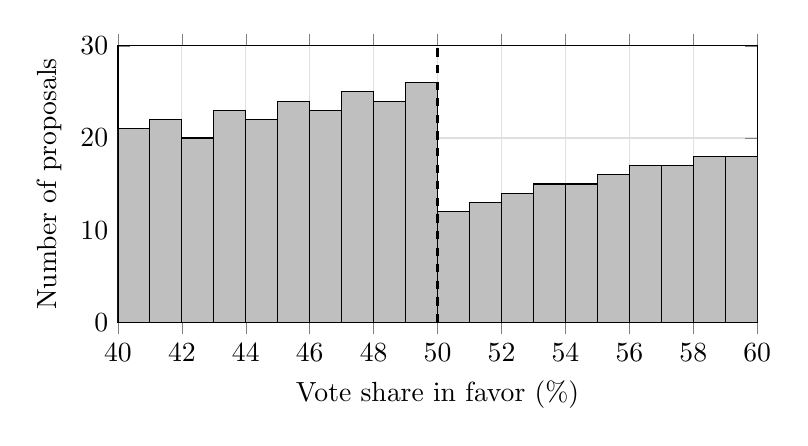
\begin{tikzpicture}
\begin{axis}[
  width=0.8\textwidth, height=0.42\textwidth,
  ybar interval,
  x tick label as interval=false,
  xlabel={Vote share in favor (\%)},
  ylabel={Number of proposals},
  xmin=40, xmax=60, ymin=0, ymax=30,
  xtick={40,42,44,46,48,50,52,54,56,58,60},
  grid=major, grid style={gray!25},
  fill=gray!50
]
\addplot[fill=gray!50, draw=black] coordinates {
  (40,21) (41,22) (42,20) (43,23) (44,22) (45,24) (46,23) (47,25) (48,24) (49,26)
  (50,12) (51,13) (52,14) (53,15) (54,15) (55,16) (56,17) (57,17) (58,18) (59,18) (60,18)
};
\draw[dashed, thick] (axis cs:50,0) -- (axis cs:50,30);
\end{axis}
\end{tikzpicture}
\caption*{Figure B1: Distribution of vote share on rotating-employee-seat proposals, 40 to 60 percent. Bins are one percentage point wide. The dashed line marks the 50 percent passage threshold. $N = 385$ proposals.}
\end{figure}

Table B1 reports a local linear estimate with a triangular kernel at the MSE-optimal bandwidth of 6.0 percentage points (Calonico, Cattaneo, and Titiunik 2014), with conventional and robust bias-corrected inference. The outcome is the layoff rate in the two years after the meeting. Standard errors are clustered by firm. Narrow passage is associated with a layoff rate 1.6 percentage points lower. This parallels the main result and suggests that employee voice at the board level, like voice through a council, slows workforce reductions (see also Cu\~nat, Gin\'e, and Guadalupe 2012 on close governance votes).

\begin{table}[htbp]
\centering
\begin{threeparttable}
\caption*{Table B1: Close votes on rotating-employee-seat proposals and the layoff rate}
\begin{tabular}{lc}
\toprule
 & (1) \\
\midrule
Proposal passed & $-$1.6** \\
 & (0.7) \\
Robust bias-corrected $p$-value & 0.04 \\
\midrule
Bandwidth (percentage points) & 6.0 \\
Proposals below / above threshold & 144 / 85 \\
Clusters (firms) & 173 \\
\bottomrule
\end{tabular}
\begin{tablenotes}\footnotesize
\item \emph{Notes:} Dependent variable: layoff rate in the two years after the shareholder meeting, in percent. Local linear regression with a triangular kernel. Conventional standard error clustered by firm in parentheses. *** $p<0.01$, ** $p<0.05$, * $p<0.10$.
\end{tablenotes}
\end{threeparttable}
\end{table}

\end{document}
